This section provides examples of using \texttt{EE-UQ} for uncertainty
quantification of structural analysis models used in earthquake
engineering. Results of each model are verified against results
obtained using other tools.

\section{Two-Dimensional Portal Frame subjected to Gravity and Earthquake Loading}
In this example, a simple 2D portal frame model is used to verify the
results of \texttt{EE-UQ}. The model is a linear elastic single-bay,
single-story model of a reinforced concrete portal frame, as shown in
\autoref{fig:figure20}. The analysis of this model considers both
gravity loading and lateral earthquake loading due to the El Centro
earthquake (Borrego Mountain 04/09/68 0230, El Centro ARRAY \#9, 270).
The original model and ground motion used in this example were
obtained from
\href{http://opensees.berkeley.edu/wiki/index.php/OpenSees_Example_1b._Elastic_Portal_Frame}{example 1b} on the \texttt{OpenSees} website, 
and were modified to scale the ground motion record from gravity units, $g$,
to the model units, $in/s^2$. Files for this example are included
with the release of the software and are available in the Examples
folder in a subfolder called \texttt{PortalFrame2D}.

\begin{figure}[!htbp]
  \centering {
    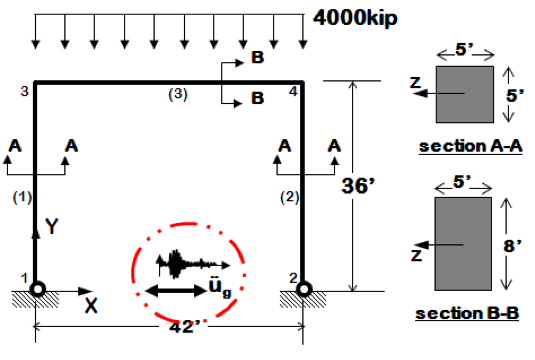
\includegraphics[width=0.8\textwidth]
    {figs/Figure20.png} }
  \caption{Two-dimensional portal frame model subjected to gravity and earthquake loading}
  \label{fig:figure20}
\end{figure}

To introduce uncertainty in the model, both mass and young’s modulus
are assumed to be normally distributed random variables with means and
standard deviation values shown in \autoref{tab:uncertainty}. In this
example, the model will be sampled with the Latin Hypercube sampling
method using both \texttt{EE-UQ} and a Python script
(\texttt{PortalFrameSampling.py}) and response statistics from both
analyses are compared.

\begin{table}[hbt!]                       
  \centering
\begin{adjustbox}{max width=\textwidth}            
  \begin{tabular}{lllll}                    
    \toprule          
      Uncertain Parameter & 	Distribution	 &  Mean  &  Standard Deviation \\ \hline
	Nodal Mass, m [kip]	 & Normal & 	5.18	 & 1.0 \\ \hline
	Young’s Modulus, E [ksi] & 	Normal	 & 4227	 & 500.0 \\ \hline
  \end{tabular}
\end{adjustbox}
  \caption{Uncertain parameters defined in the portal frame model}             
  \label{tab:uncertainty}                 
\end{table}

Modeling uncertainty using \texttt{EE-UQ} can be done using the
following steps:
\begin{enumerate}
\item	 Start \texttt{EE-UQ}, click on the simulation tab (SIM) in the left bar to open a building simulation model. Click on choose button in the input script row:

\begin{figure}[!htbp]
  \centering {
    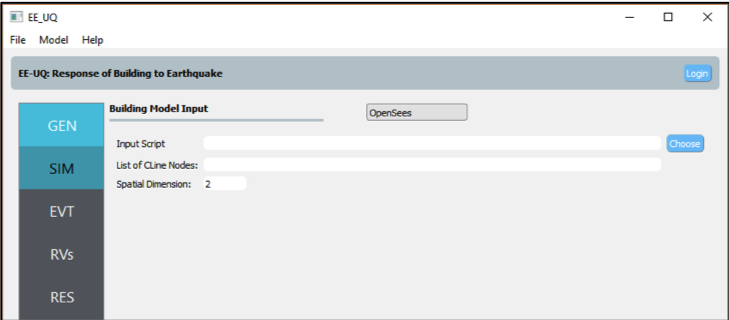
\includegraphics[width=0.8\textwidth]
    {figs/Figure21.png} }
  \caption{Choose building model}
  \label{fig:figure21}
\end{figure}

\item	 Choose the model file \texttt{Portal2D-UQ.tcl} from PortalFrame2D example folder.
\begin{figure}[!htbp]
  \centering {
    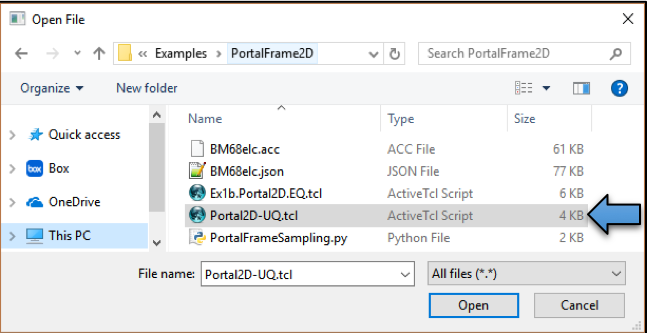
\includegraphics[width=0.8\textwidth]
    {figs/Figure22.png} }
  \caption{Choose tcl file}
  \label{fig:figure22}
\end{figure}


\item	 In the list of Clines Nodes edit box, enter “1, 3”. This indicates to \texttt{EE-UQ} that nodes 1 and 3 are the nodes used to obtain EDP at different floor levels (i.e. base and first floor).
\begin{figure}[!htbp]
  \centering {
    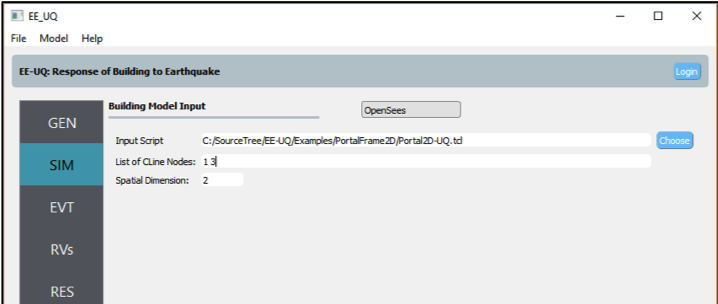
\includegraphics[width=0.8\textwidth]
    {figs/Figure23.png} }
  \caption{Select nodes}
  \label{fig:figure23}
\end{figure}

\item Click on the event tab (EVT) in the left bar to open the earthquake event specification tab, select Multiple Existing for loading Type. Click on the add button to add an earthquake event. 
Then click on the choose button to select the event file.
\begin{figure}[!htbp]
  \centering {
    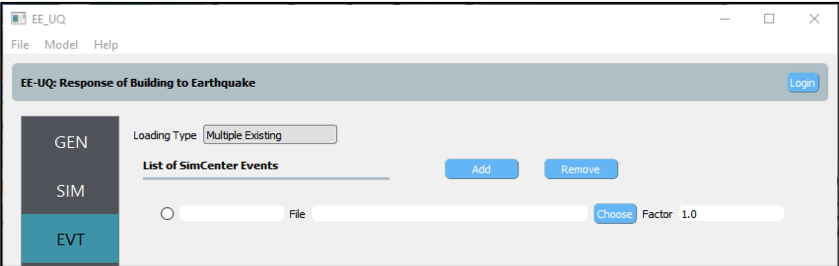
\includegraphics[width=0.8\textwidth]
    {figs/Figure24.png} }
  \caption{Work on EVT tab}
  \label{fig:figure24}
\end{figure}

\item Choose the event file (\texttt{BM68elc.json}) for El Centro earthquake provided in the portal frame 2D example folder.
\begin{figure}[!htbp]
  \centering {
    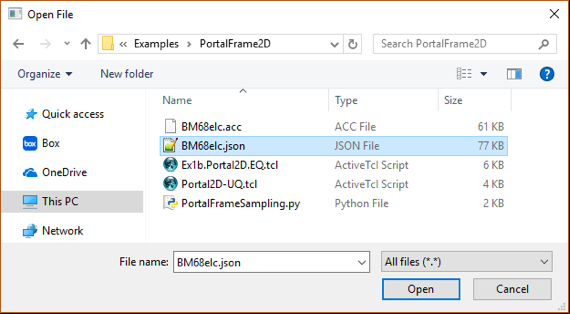
\includegraphics[width=0.8\textwidth]
    {figs/Figure25.png} }
  \caption{Choose event file}
  \label{fig:figure25}
\end{figure}

\item Now select the random variables tab (RVs) from the left bar, change the random variables types to normal and set the mean and standard deviation values of the floor mass and
Young’s modulus.  Notice that \texttt{EE-UQ} has automatically
detected parameters defined in the \texttt{OpenSees} tcl file using the pset
command and defined them as random variables.
\begin{figure}[!htbp]
  \centering {
    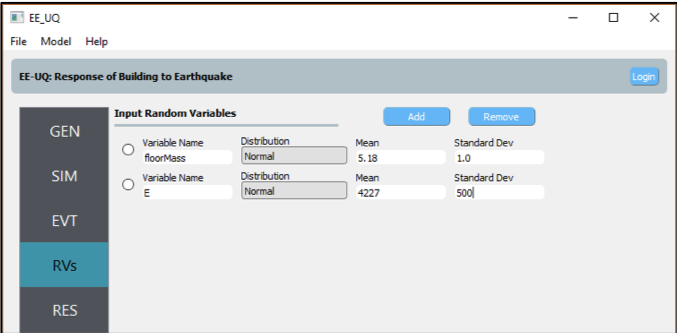
\includegraphics[width=0.8\textwidth]
    {figs/Figure26.png} }
  \caption{Work on RVs tab}
  \label{fig:figure26}
\end{figure}

\item Now click on run, set the analysis parameters, working directory and applications directory and click submit to run the analysis. 
If everything ran successfully the program will automatically open the results tab showing the summary of results (\autoref{fig:figure27}).
\begin{figure}[!htbp]
  \centering {
    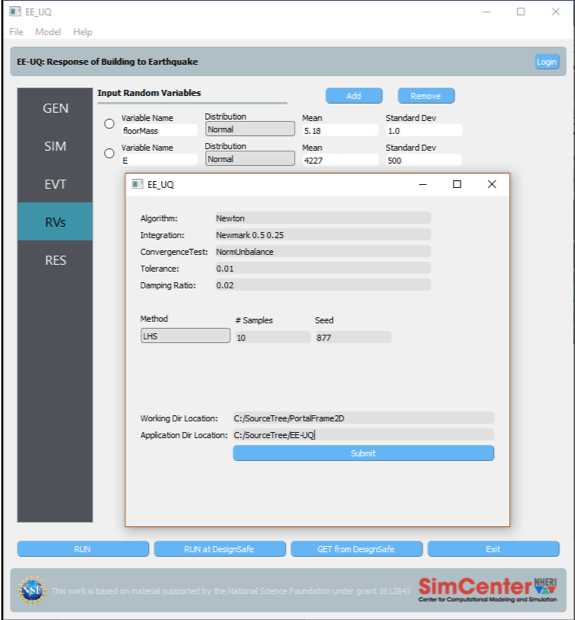
\includegraphics[width=0.8\textwidth]
    {figs/Figure27.png} }
  \caption{Run}
  \label{fig:figure27}
\end{figure}

\end{enumerate}


\subsection{Verification Script}
A verification script (Listing 1) for propagating the uncertainty was
developed in Python and is included in the example folder.  The script
creates 1000 samples for both the Young’s modulus and mass values
using Latin Hypercube sampling, then modifies the \texttt{OpenSees} model, runs
it and stores the output.  After all the model samples are processed,
the script will compute and output the mean and standard deviation
values of the peak floor acceleration and peak drift.


\begin{python}[caption=Python script for analyzing the portal frame model with uncertain parameters]
import numpy as np
import os
import shutil
import subprocess
from pyDOE import *
from scipy.stats.distributions import norm

#Setting number of samples
nSamples = 1000

#Creating latin hyper cube designs
design = lhs(2, samples=nSamples)

#Sampling Young's Modulus and Mass
ESamples = norm(loc=4227, scale=500.0).ppf(design[:,0])
mSamples = norm(loc=5.18, scale=1.0).ppf(design[:,1])

#Initializing output arrays
PFA = []
PID = []
#Reading OpenSees Model
with open ("Ex1b.Portal2D.EQ.tcl", "r") as portalFrameFile:
    portalFrameModel = portalFrameFile.read()

    #Looping through the samples and creating modified models
    for i in range(nSamples):
        sampleName = str(i+1)
        if(os.path.exists(sampleName) and os.path.isdir(sampleName)):
            shutil.rmtree(sampleName)

        os.mkdir(sampleName)
        shutil.copy('BM68elc.acc', sampleName)

        #Modifying the model using sample E and m values
        with open (sampleName + '/Ex1b.Portal2D.EQ.tcl' , "w+") as modifiedFile:
            modifiedModel = portalFrameModel.replace('pset floorMass 5.18', 'pset floorMass ' + str(mSamples[i]))
            modifiedModel = modifiedModel.replace('pset E 4227', 'pset E ' + str(ESamples[i]))
            modifiedFile.write(modifiedModel)

        #Running OpenSees
        subprocess.Popen("OpenSees Ex1b.Portal2D.EQ.tcl", shell=True, cwd=sampleName).wait()

        #Reading Peak Floor Acceleration
        with open (sampleName + '/PFA.out' , "r") as pfaFile:
            PFA.append(float(pfaFile.readlines()[2]))

        #Reading Peak Floor Acceleration
        with open (sampleName + '/PID.out' , "r") as pidFile:
            PID.append(float(pidFile.readlines()[2]))

        #Cleaning up
        shutil.rmtree(sampleName)

#Printing results
print 'Mean Peak Floor Acceleration: ', np.mean(PFA)
print 'Peak Floor Acceleration Std. Dev: ', np.std(PFA)

print 'Mean Peak Drift: ', np.mean(PID)
print 'Peak Drift Std. Dev.: ', np.std(PID)
\end{python}

\subsection{Verification of Results}
In this section, the results produced for the portal frame
by \texttt{EE-UQ} are verified against the results of running the same
problem using the Python script.  Running the uncertainty
quantification problem on the local computer produces the results
shown in \autoref{fig:figure28} Running the analysis using the
sampling Python script produces the results shown
in \autoref{fig:figure29}.  Both results (Mean and standard deviation
values of EDPs) are compared in \autoref{tab:edp} and are shown to be in good
agreement.

\begin{figure}[!htbp]
  \centering {
    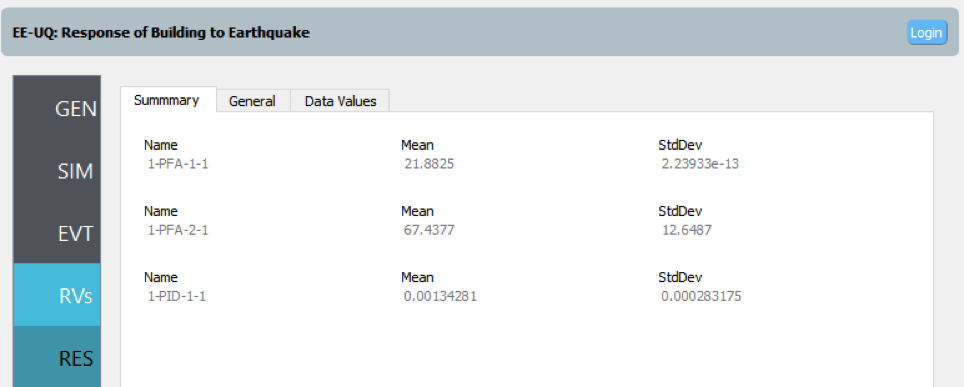
\includegraphics[width=0.8\textwidth]
    {figs/Figure28.png} }
  \caption{Outputs from \texttt{EE-UQ}}
  \label{fig:figure28}
\end{figure}


\begin{figure}[!htbp]
  \centering {
    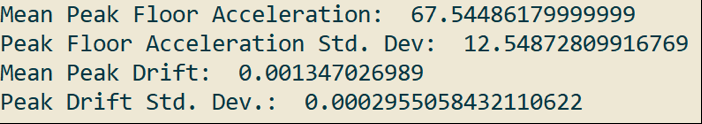
\includegraphics[width=0.8\textwidth]
    {figs/Figure29.png} }
  \caption{Outputs from PortalFrameSamplying.py script}
  \label{fig:figure29}
\end{figure}




\begin{table}[hbt!]                 
  \centering
\begin{adjustbox}{max width=\textwidth}            
  \begin{tabular}{lllll}                    
    \toprule          
      Engineering Demand Parameter &	 & \texttt{EE-UQ}	& Python Script	 & Percent Difference [\%]  \\ \hline
    
	\multirow{2}{*}{Peak Floor Acceleration [in/$s^2$]} 
	 & Mean &	67.4377	& 67.5448	& 0.16 \\
      & Std. Dev.	& 12.6487	 & 12.5487	& 0.8 \\ \hline
      
      \multirow{2}{*}{Peak Story Drift [x10-3 in]} 
      & Mean &	1.3428 &	1.347 &	0.3 \\
      & Std. Dev.	& 0.2832 &	0.2955	& 4.1	 \\

      \bottomrule      
                            
  \end{tabular}
\end{adjustbox}
  \caption{Engineering demand parameters verification}             
  \label{tab:edp}                 
\end{table}

\section{Response Spectrum Calculation using Stochastic Ground Motion Model}
The purpose of this analysis is to verify that \texttt{EE-UQ} is able
to reproduce the correct pseudo-acceleration response spectrum when
using synthetic acceleration time histories generated using the
stochastic ground motion model option as the seismic event. The maximum
pseudo-acceleration for a single-degree-of-freedom system with varying
natural frequencies calculated by \texttt{EE-UQ} is compared to the
values predicted by \texttt{smelt} as well as the geometric mean
of the four NGA-West2 ground motion prediction equations (GPMEs)
that account for soil sites. 

The single-degree-of-freedom system was input using the MDOF option as
the Building Model Input in \texttt{EE-UQ}. Here, the mass was set to
unity and the damping ratio to 5\%. The story stiffness was modified
to set the natural frequency of the system in order to calculate the
response spectrum. The structural response was calculated for 10
sample synthetic acceleration time histories for each structural
period and compared to those from \texttt{smelt} and the GMPEs, as
shown in \autoref{fig:stochastic_validation}. As can be seen in this
figure, the spectral response calculated by \texttt{EE-UQ} falls
within the mean plus/minus one sigma bounds of the GMPEs and
\texttt{smelt} while tending toward the mean. This produces the
expected result as \texttt{EE-UQ} is calling \texttt{smelt} in the
backend to generate the synthetic motions. The full validation of
\texttt{smelt} in implementing the predictive stochastic model
proposed by Vlachos et al. (2018) \cite{vlachos2018predictive} can be
found in the
\href{https://github.com/shellshocked2003/Stochastic-Loading-Module/blob/master/README.md}{library
  documentation}.

\begin{figure}[!htbp]
  \centering {
    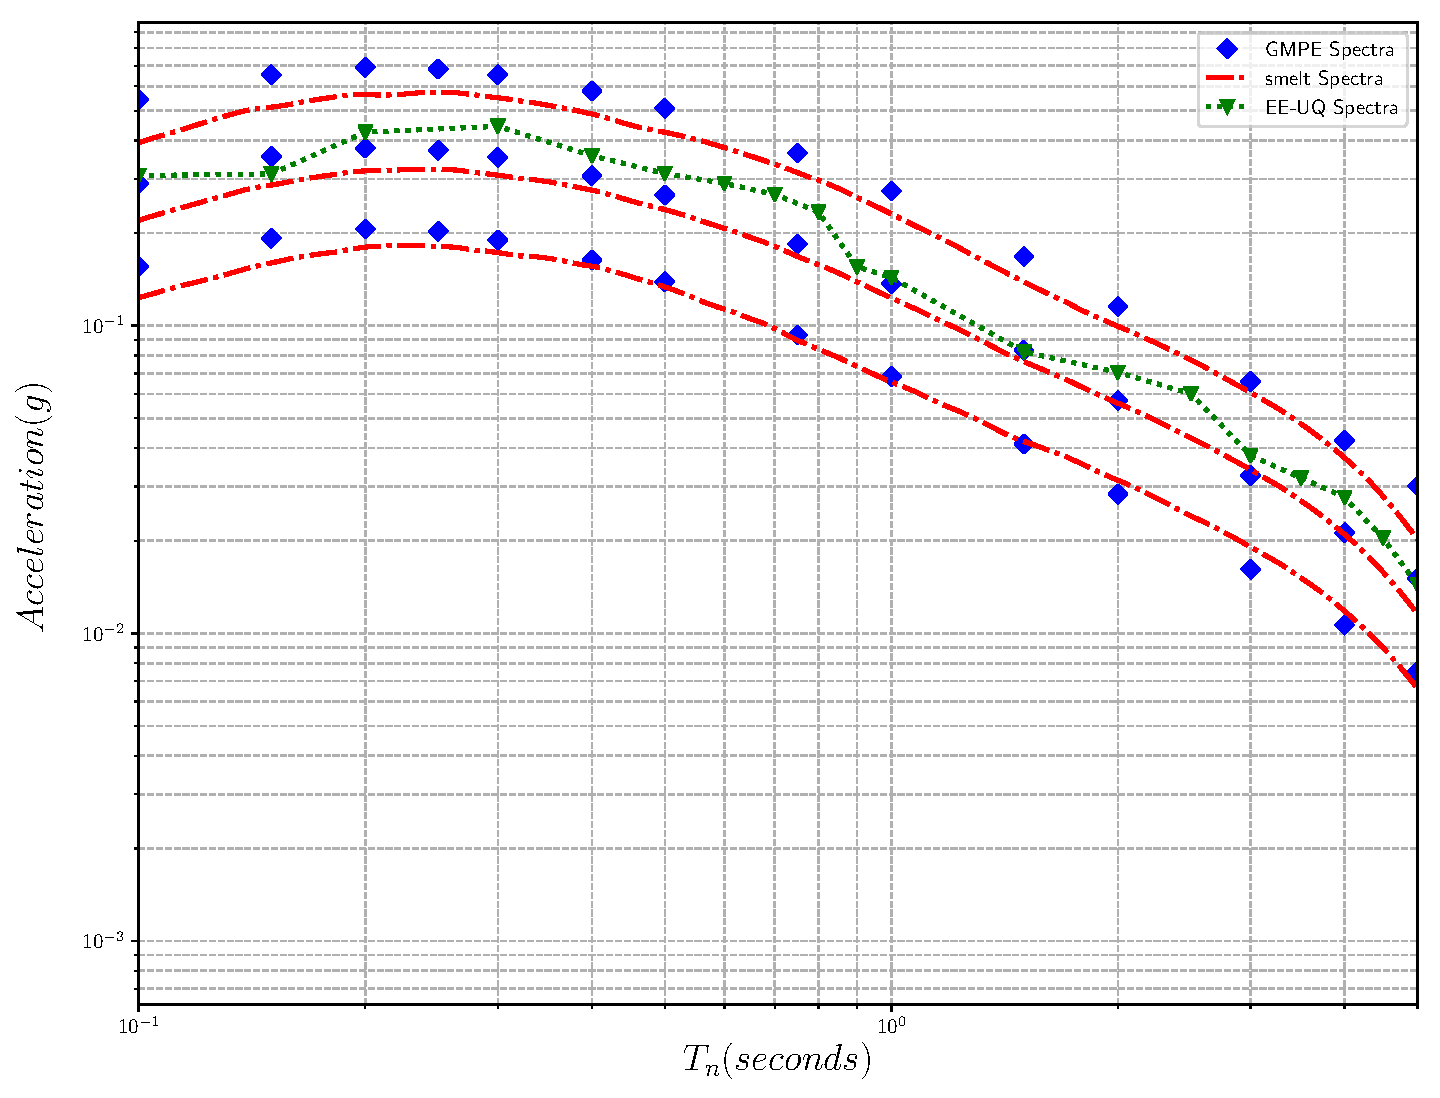
\includegraphics[width=0.8\textwidth]
    {figs/M65R20V400.pdf} }
  \caption{Response Spectra generated using NGA-West2 GMPEs,
    \texttt{smelt} \& \texttt{EE-UQ} for $M_W = 6.5$, closest-to-site
    distance $R = 20km$, and average shear-wave velocity $V_{s_{30}} =
    400m/s$. The \texttt{smelt} and GMPE spectra show the mean and
    mean plus/minus one logarithmic standard deviation. The GMPE
    spectra are based on the geometric mean of the four NGA-West2
    models that account for site soil conditions. The \texttt{smelt}
    spectra are based on an ensemble of 1000 synthetic ground
    motions. \texttt{EE-UQ} response values are based on the mean
    pseudo-acceleration for 10 synthetic ground motion samples per
    period, $T_n$}
  \label{fig:stochastic_validation}
\end{figure}

